\section{Flight controller}\label{firmware}
\subsection{Firmware}
\label{fc-firmware}
Flight controller (FC) firmware is the software that runs on a flight controller and controls the operation of an FPV drone. It affects flight performance and features, and different firmware options offer various advantages and disadvantages for different flying styles and preferences. \cite{firmware-FC}

There are mainly two firmwares \cite{firmware-FC} to choose from for autonomous flying today:
\begin{itemize}
  \item INAV
  \item ArduPilot
\end{itemize}

ArduPilot is perhaps the most popular open-source autopilot software suite. It supports a variety of vehicles, including quadcopters, planes, rovers, ground vehicles, even RC submarines.

ArduPilot is known for its extensive features and customization options, making it a good choice for advanced pilots and developers. It supports both autonomous and manual control modes, GPS waypoint navigation, and various sensors like barometers and magnetometers. \cite{firmware-FC}

\begin{figure}[!htb]
    \centering
    
\includegraphics[width=\textwidth]{fig/ardupilot_logo.jpg}
    \caption{ArduPilot logo, from ardupilot.org \protect\cite{documentation-ArduPilot}}
\end{figure}

ArduPilot was chosen as baseline firmware since it is a long-standing open-source project that's well-documented \cite{documentation-ArduPilot} compared to INAV \cite{github-wiki-INAV}. ArduPilot is also the only firmware officially supported by the MATEKSYS Flight Controller H743-SLIM (ref: \ref{fc}) out of these two options.


\subsection{MAVLink}
\label{MAVLink}

MAVLink is a very lightweight messaging protocol for communicating with drones (and between onboard drone components).

MAVLink follows a modern hybrid publish-subscribe and point-to-point design pattern: Data streams are sent / published as topics while configuration sub-protocols such as the mission protocol or parameter protocol are point-to-point with retransmission. \cite{documentation-MAVLink}

\iffalse
As ArduPilot natively supports MAVLink  we wanted to take advantage of this and have employed the MAVLink protocol via a ROS2-node running a program utilizing the "pymavlink" python-libraries for serial communcation between the FC and the SBC.
\fi

\subsubsection{MAVLink Commands}
\label{MAVLink-commands}
With the help of the relatively low-level "Pymavlink" Python-library we're able to send and receive messages to and from an ArduCopter-flashed flight controller. To do this, first import "mavutil" from the "pymavlink" libraries and establish a connection and wait for a heartbeat from the flight controller:
\begin{lstlisting}[language=PythonPlus]
from pymavlink import mavutil

# Tries to establish connection on Raspberry Pi serial UART:
the_connection = mavutil.mavlink_connection("/dev/ttyACM0", baud=57600)
the_connection.wait_heartbeat()
\end{lstlisting}

After "the\_connection" is successfully initialized its from here on possible to communicate with the flight controller.
\newpage
As an example, to command the flight controller to change mode, arm throttle, and take off can be done by encoding each of these three desired commands in each of their respective "COMMAND\_LONG" messages, including all the command's parameters, as per the MAVLink.io\cite{documentation-MAVLink} documentation:
\begin{lstlisting}[language=PythonPlus]
# Sets flight controller flight mode to "GUIDED":
the_connection.mav.command_long_send(
    the_connection.target_system,           # Established after heartbeat
    the_connection.target_component,        # Established after heartbeat
    mavutil.mavlink.MAV_CMD_DO_SET_MODE,    # Command to be sent
    0,                                      # Confirmation bit
    1, 4, 0, 0, 0, 0, 0)                    # The command's 7 parameters

# Arms the throttle to allow for motors to spin:
the_connection.mav.command_long_send(
    the_connection.target_system,
    the_connection.target_component,
    mavutil.mavlink.MAV_CMD_COMPONENT_ARM_DISARM,
    0,
    1, 0, 0, 0, 0, 0, 0)

# Takes off to 5 metres above ground level:
the_connection.mav.command_long_send(
    the_connection.target_system,
    the_connection.target_component,
    mavutil.mavlink.MAV_CMD_NAV_TAKEOFF,
    0,
    0, 0, 0, 0, 0, 0, 5)
\end{lstlisting}

Every MAVLink command has 7 parameters that need to be set, these parameters can be looked up in the MAVLink.io\cite{documentation-MAVLink} documentation for each respective command.

\subsubsection{Manual Control Protocol}
The "MAVLink Commands" example above works fine for programmatically moving the drone on a "macro"-scale where the flight controller has GNSS-signal available. To programmatically move the drone on a "micro"-scale its possible to do this through the "MANUAL\_CONTROL"-message as per the MAVLink.io\cite{documentation-MAVLink} documentation:

\begin{lstlisting}[language=PythonPlus]
# After connection already established and heartbeat recieved:
the_connection.mav.manual_control_send(
    the_connection.target_system,   # Established after heartbeat
    x,                              # Pitch, in range [-1000,1000]
    y,                              # Roll, in range [-1000,1000]
    z,                              # Thrust, in range [-1000,1000]
    r,                              # Yaw, in range [-1000,1000]
    0)                              # Bitfield corresponding to extra
                                    # buttons, not needed and can be
                                    # set to 0 in this case
\end{lstlisting}

Note that the z-value (thrust) is in the range [-1000,1000] where -1000 is full negative thrust, 0 is no thrust and 1000 is full thrust. Most aircraft only operate in the range [0,1000] without any functionality for negative thrust. \\
Also note that the thrust can not be modified through this protocol unless the flight controller is in a flight mode that supports manual control, as per the ArduPilot.org\cite{documentation-ArduPilot} documentation.




\subsection{Drone simulation}
\label{drone_sim}
Simulation is implemented by using a Flight Dynamics Model (FDM) of the vehicle to simulate the physics involved with vehicle movement. It receives inputs from a SITL (Software in the Loop) program running the ArduPilot firmware (which are the firmware’s servo/motor outputs) and outputs vehicle status, position, velocities, etc. that result from those inputs back to the firmware simulation. Just as sensors would in the real world case. \cite{documentation-ArduPilot}

\subsubsection{SITL Simulator (Software in the Loop)}
The SITL simulator allows you to run Plane, Copter, or Rover without any hardware. It is a build of the autopilot code using an ordinary C++ compiler, giving you a native executable that allows you to test the behavior of the code without hardware. \cite{documentation-ArduPilot}

Through simulating the drone's flight controller running ArduPilot and interfacing with it through MAVLink messages we're able to test code in a safe environment before deploying it on a physical drone. With the addition of Gazebo \cite{Gazebo} we can see a 3D-rendering of the drone and its surrounding, making it ideal for controlling the simulated drone on a "micro"-scale.

\begin{figure}[!htb]
    \centering
    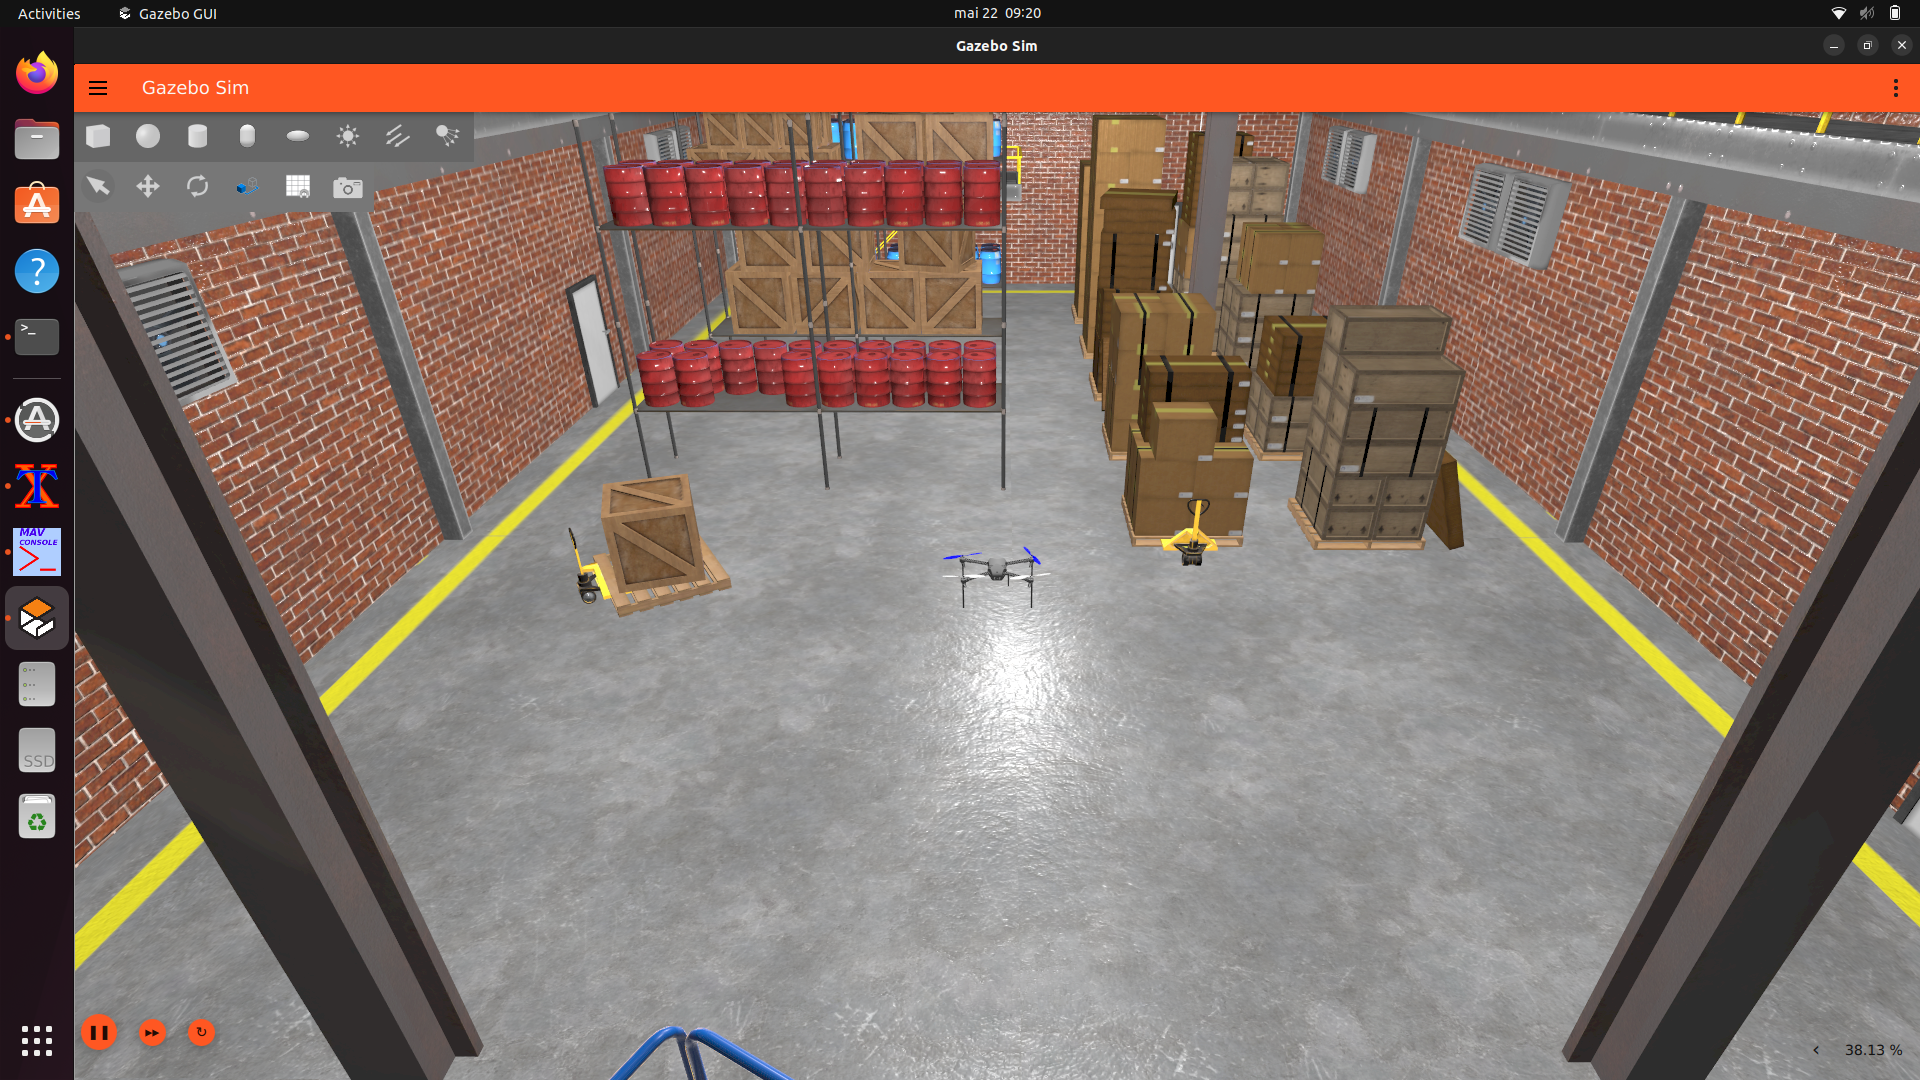
\includegraphics[width=\textwidth]{fig/sitl-gazebo.png}
    \caption{SITL with Gazebo}
\end{figure}

\newpage
\newpage

\section{Drone implementation}
\label{drone_impl}

During the project a four-rotor "quadcopter" drone was built as the project's attempt at a real-world implementation, mainly to act as a platform for our proof of concept.\\
Due to time constraints and hardware difficulties, the full context configuration with all the ROS2-nodes could not be tuned properly and therefore not implemented safely. The full context implementation was limited only to simulations with SITL.

\begin{figure}[!htb]
    \centering
    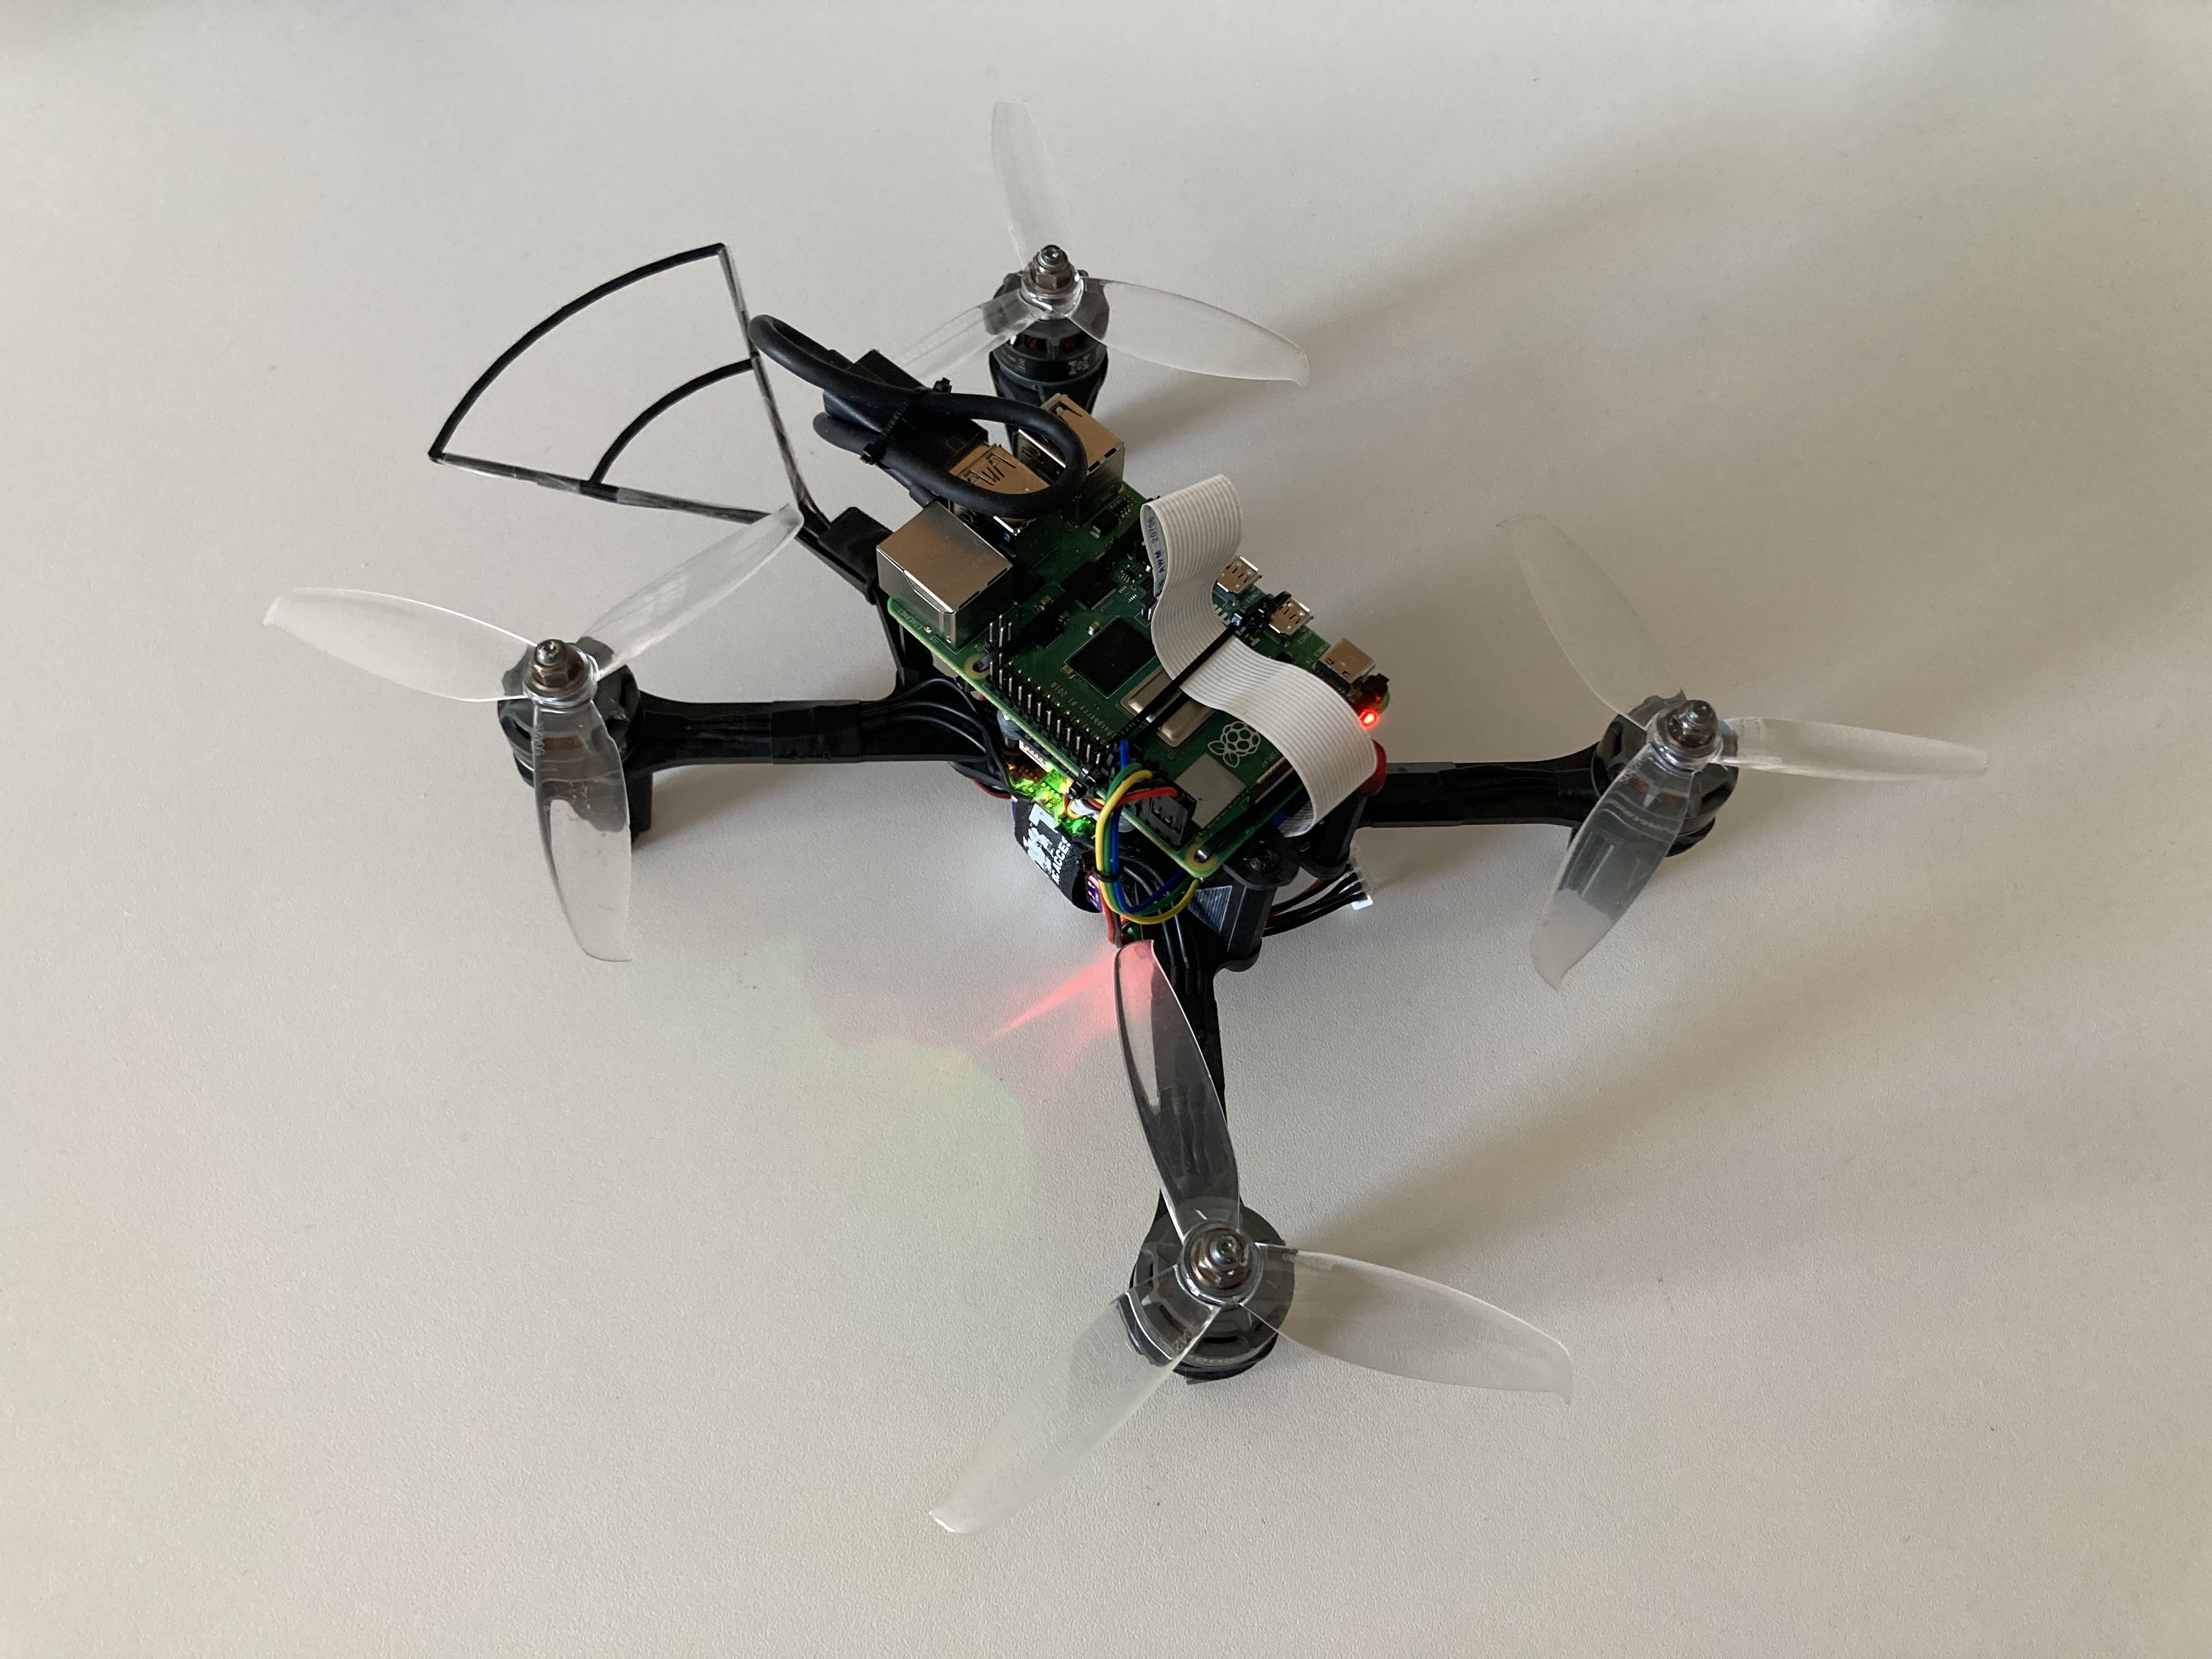
\includegraphics[width=\textwidth]{fig/drone/drone_top.jpg}
    \caption{Photo of drone from top}
\end{figure}

\newpage

\begin{figure}[!htb]
    \centering
    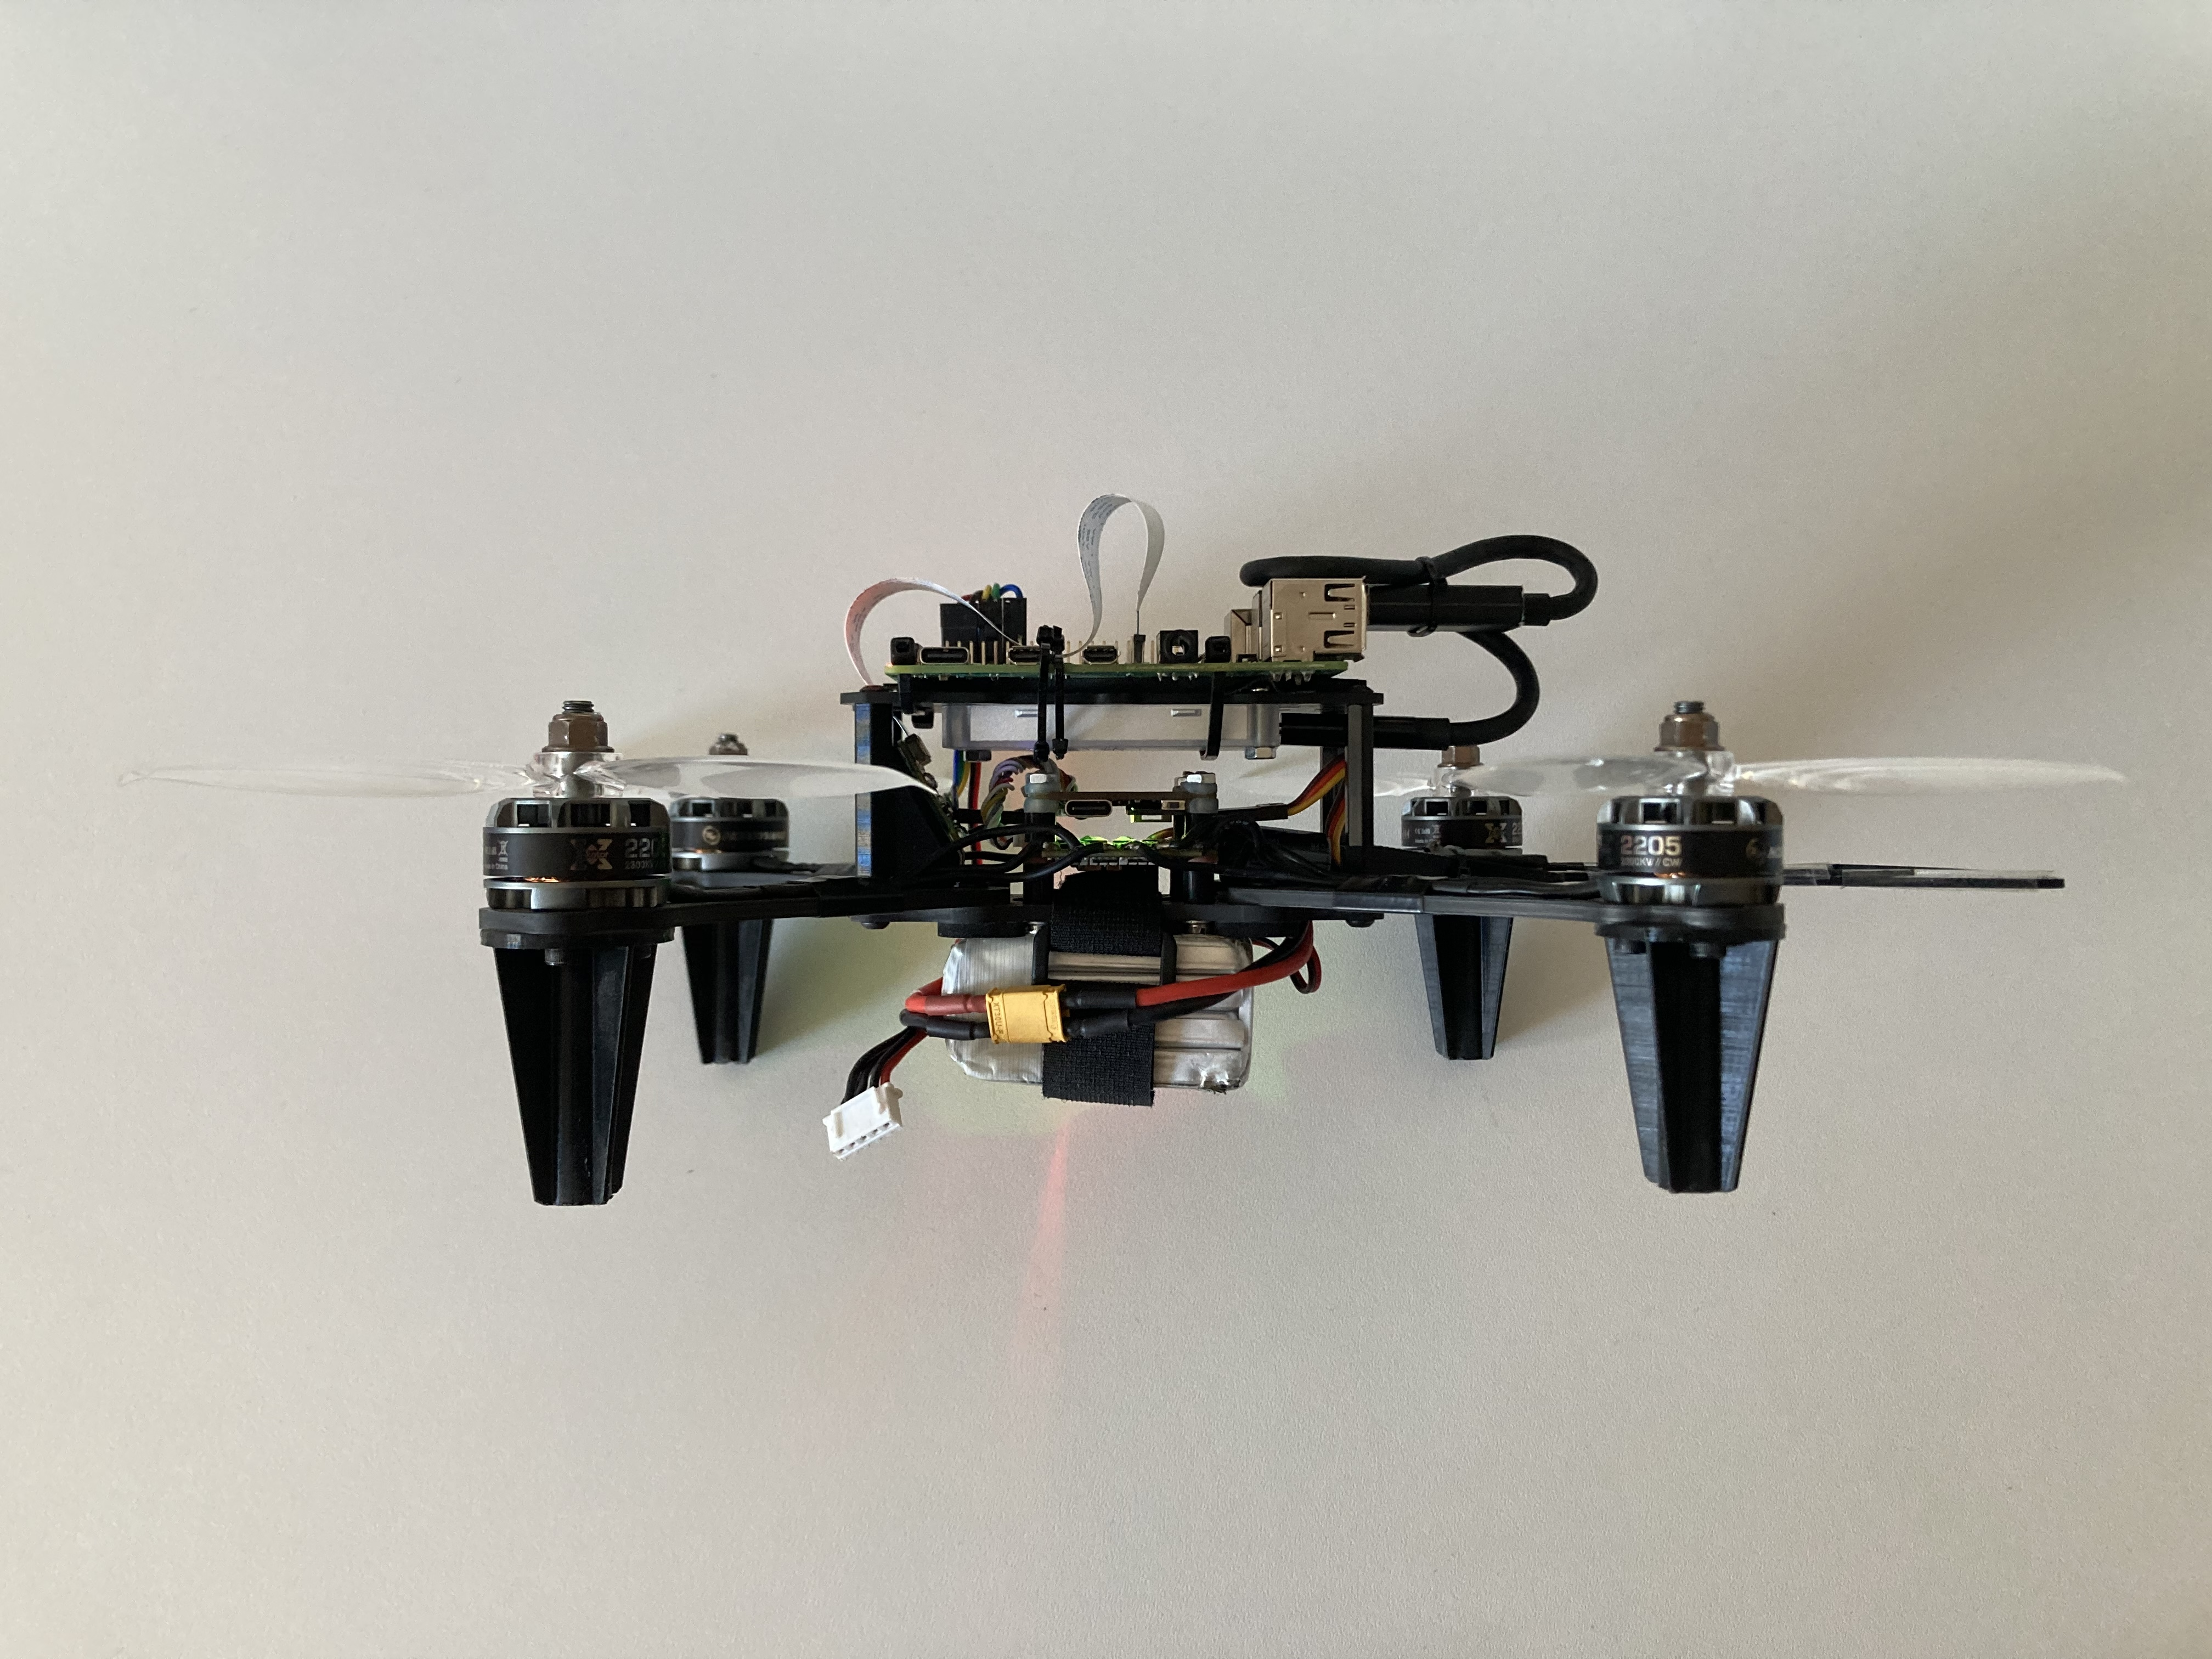
\includegraphics[width=\textwidth]{fig/drone/drone_left.jpg}
    \caption{Photo of drone from left}
\end{figure}

\newpage

\begin{figure}[!htb]
    \centering
    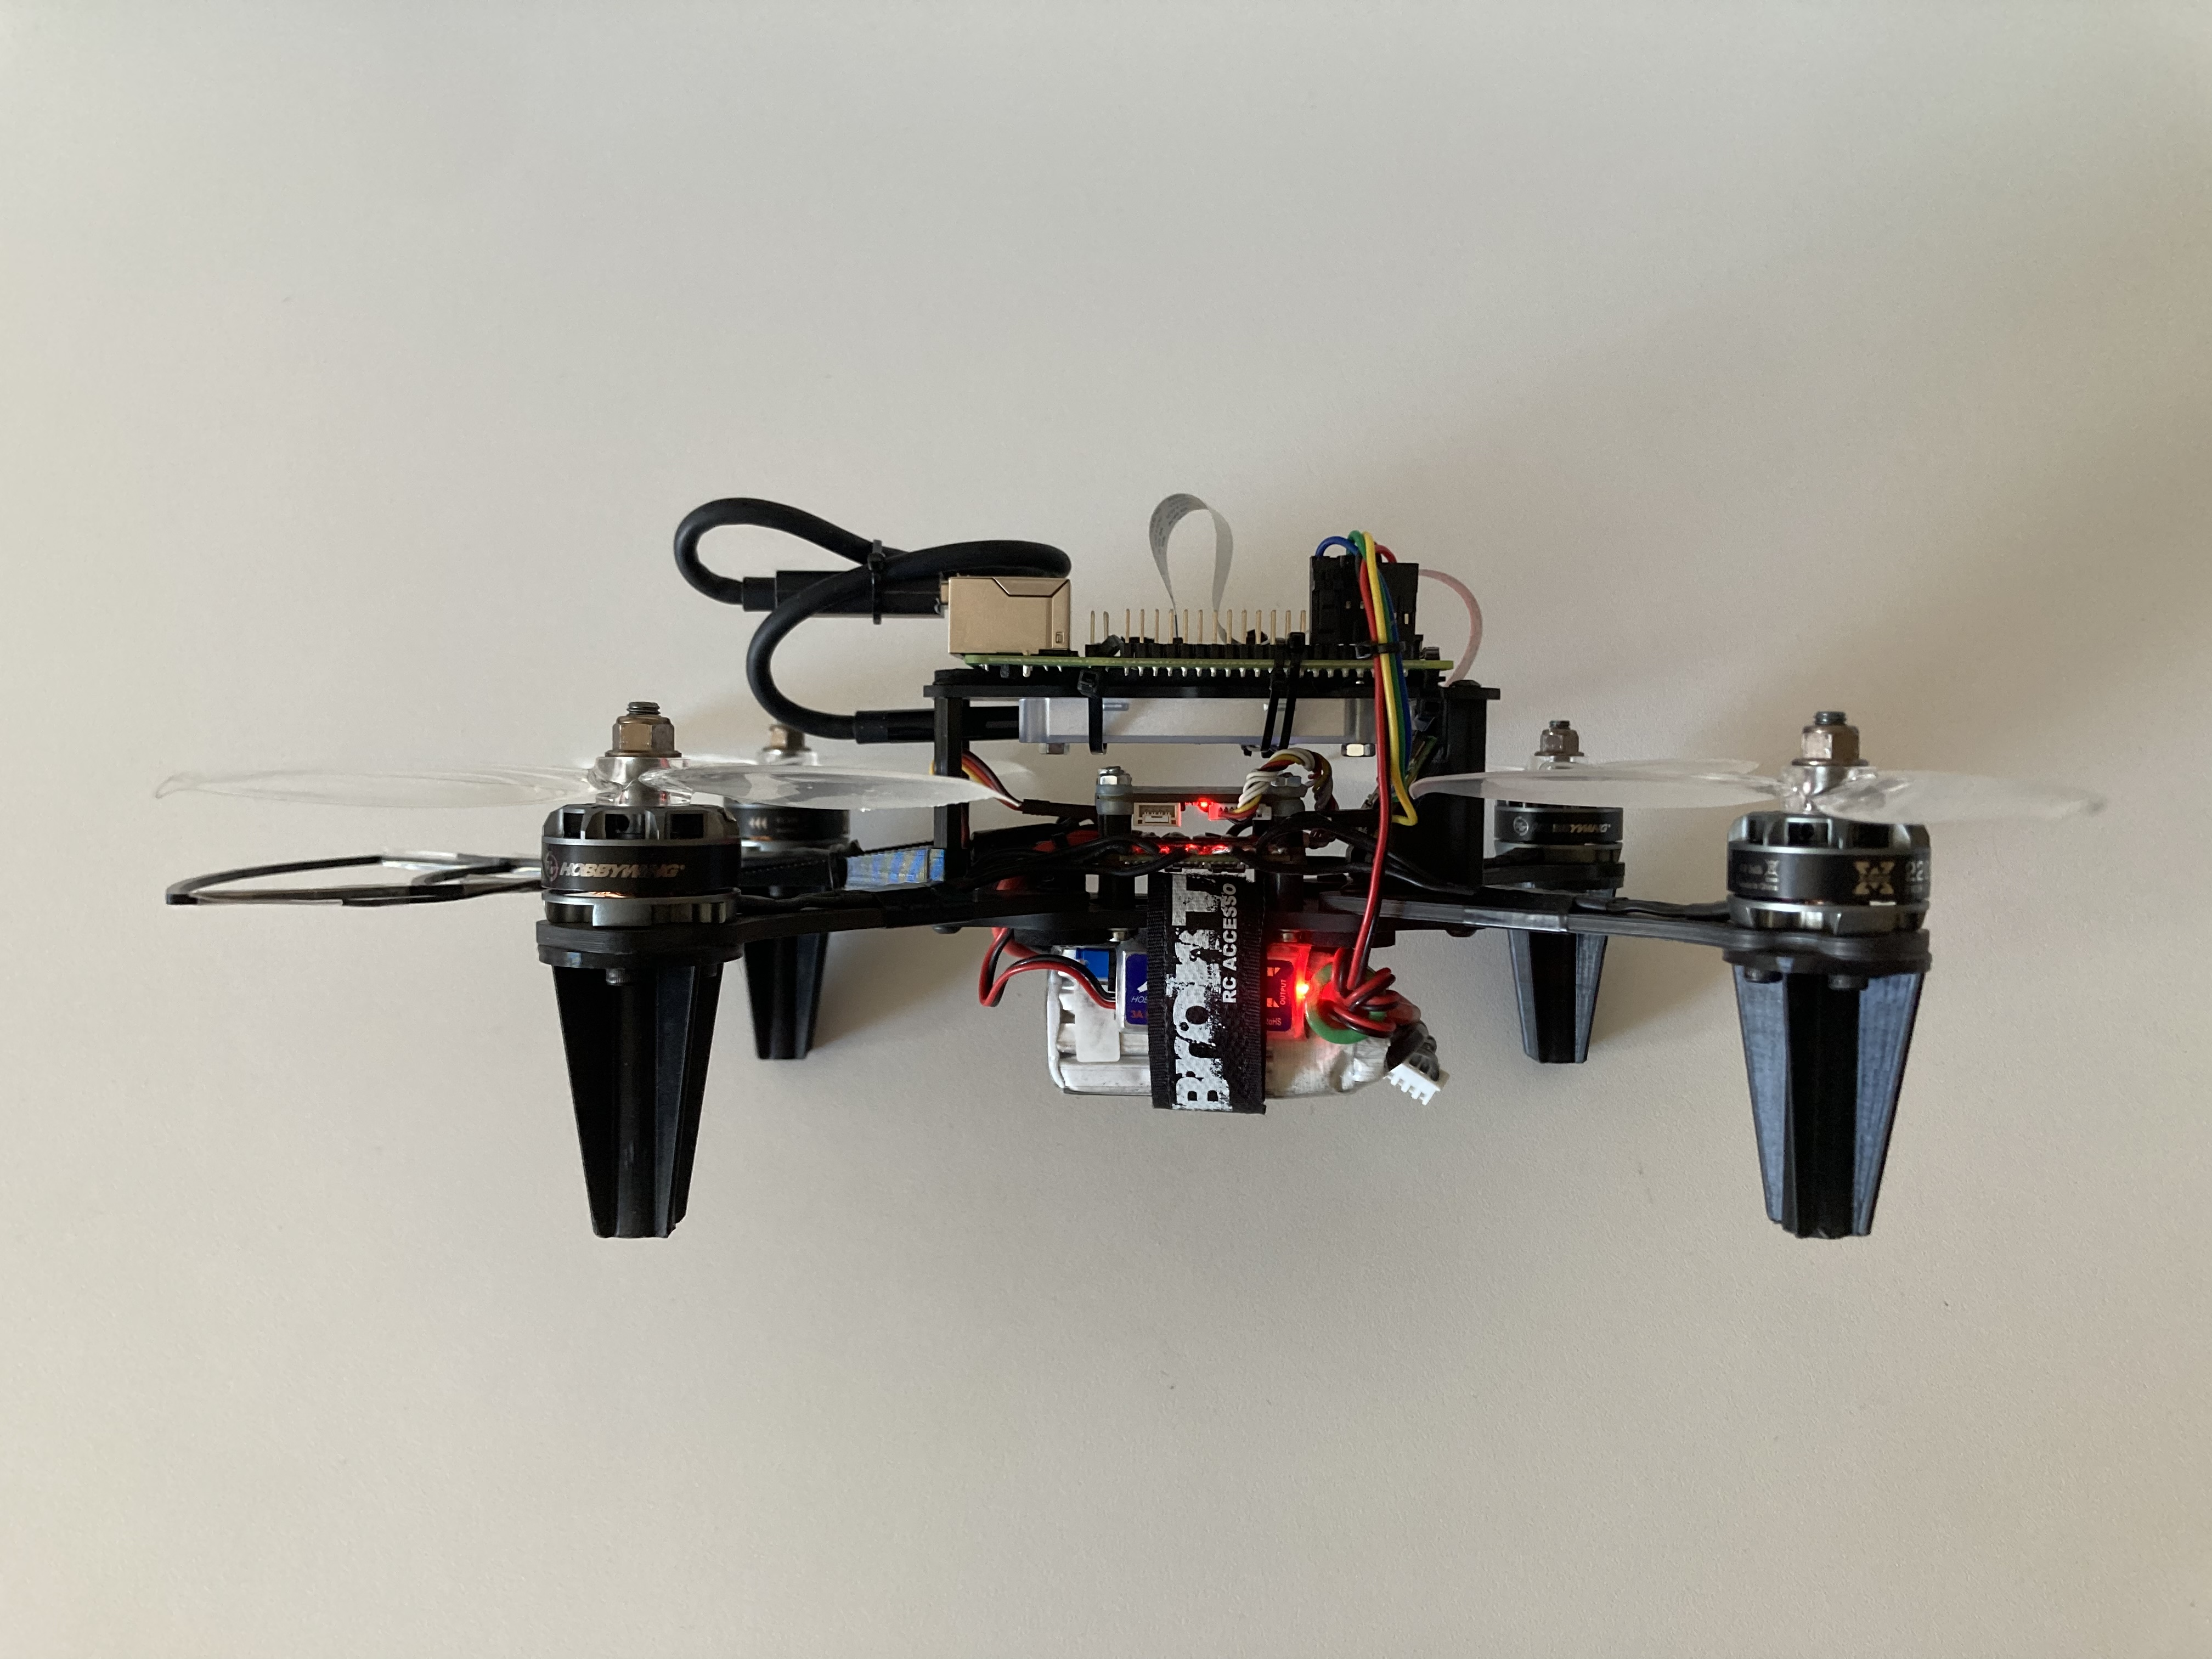
\includegraphics[width=\textwidth]{fig/drone/drone_right.jpg}
    \caption{Photo of drone from right}
\end{figure}

\newpage

\begin{figure}[!htb]
    \centering
    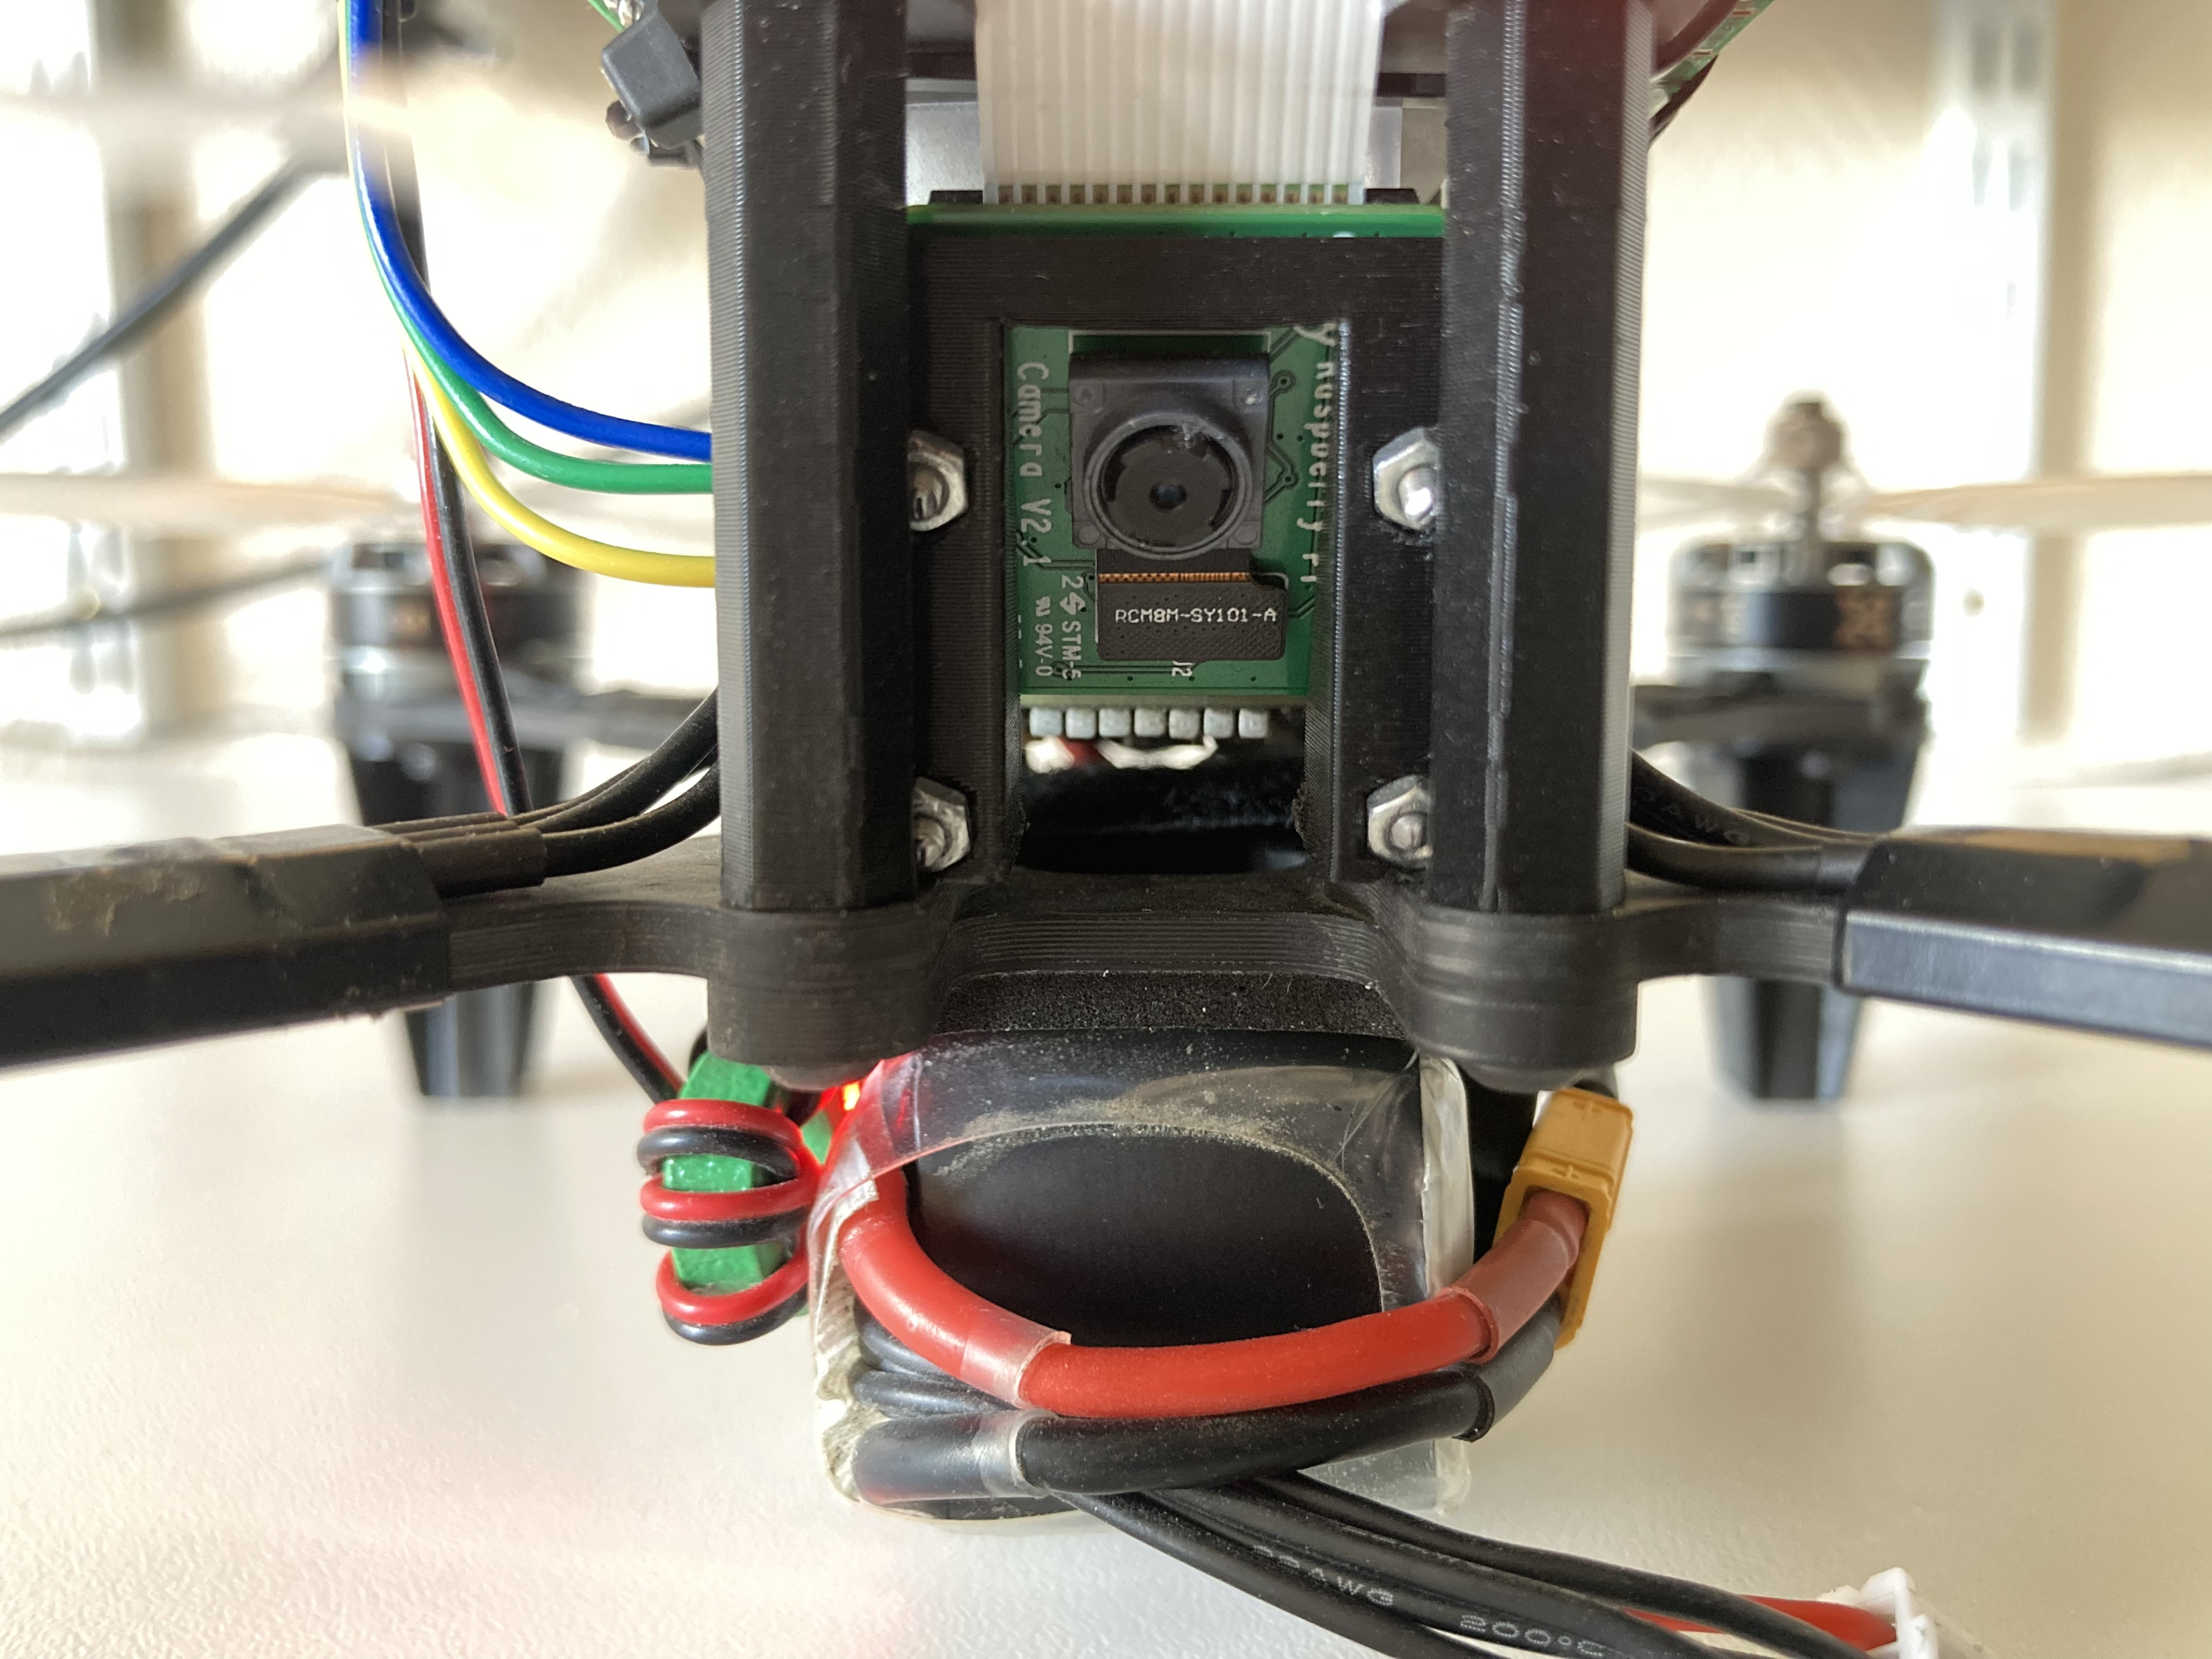
\includegraphics[width=\textwidth]{fig/drone/drone_front.jpg}
    \caption{Photo of drone from front}
\end{figure}

\newpage

\begin{figure}[!htb]
    \centering
    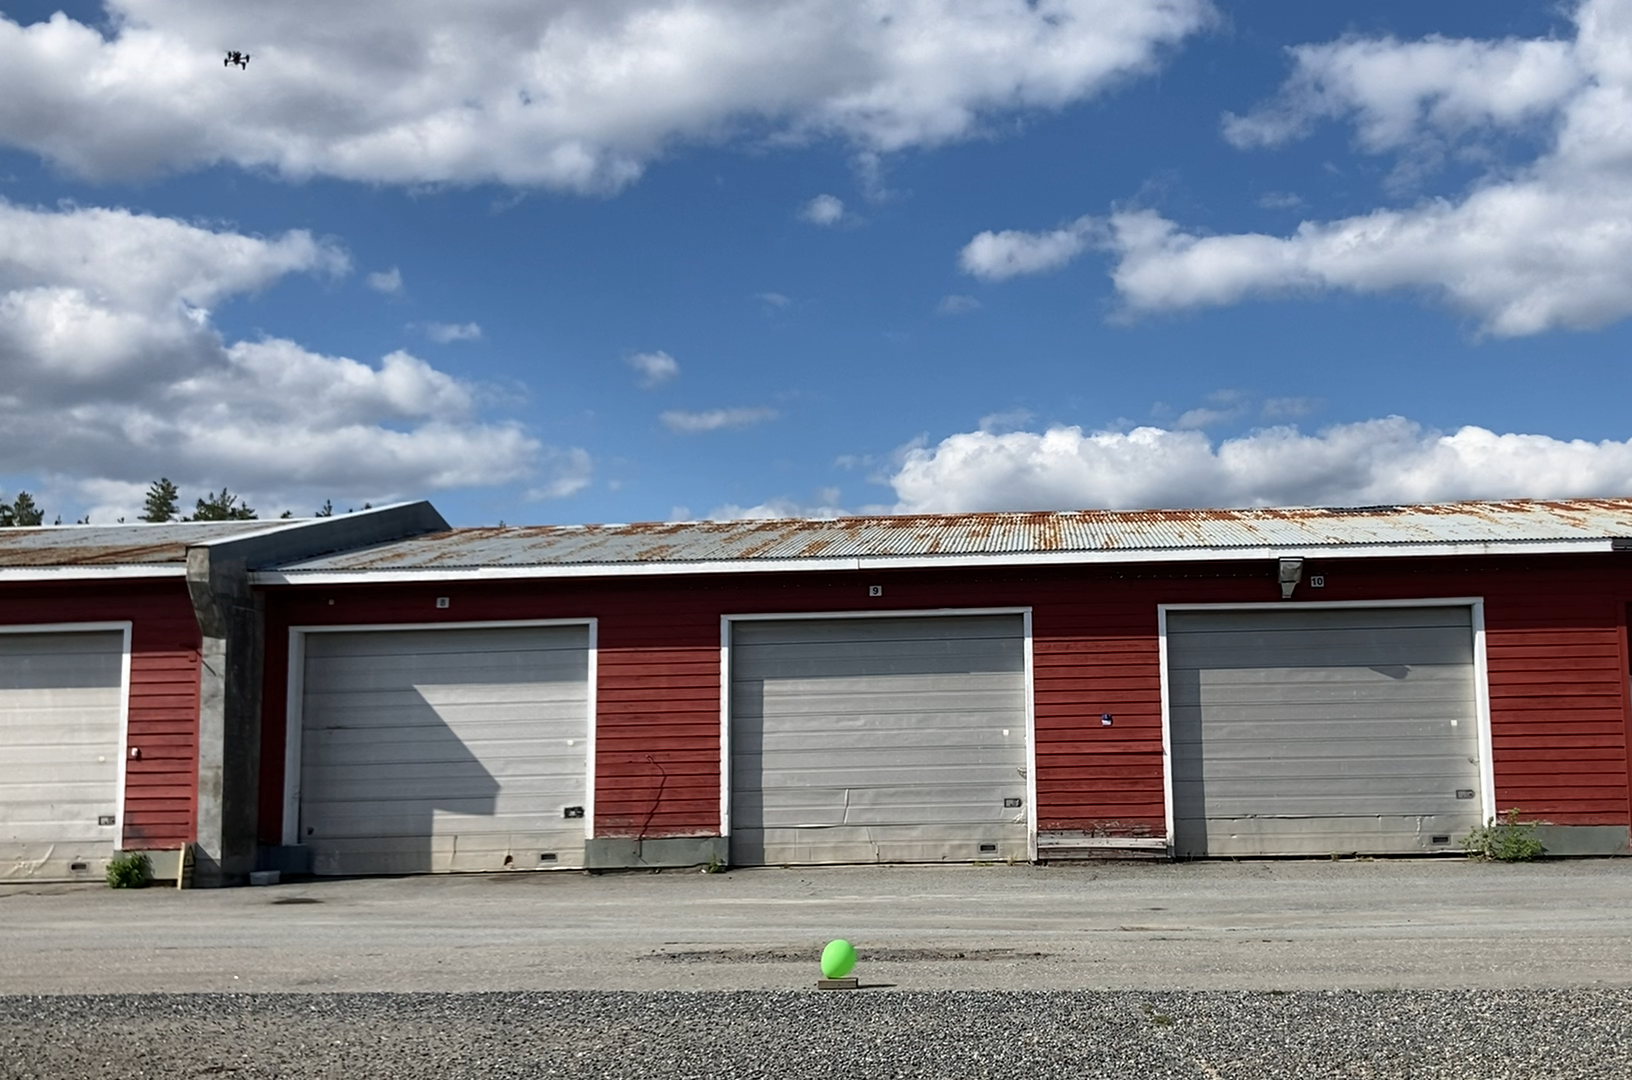
\includegraphics[width=\textwidth]{fig/drone/drone_airshot_3p.png}
    \caption{Photo of a drone hovering in the air}
\end{figure}

\newpage

\begin{figure}[!htb]
    \centering
    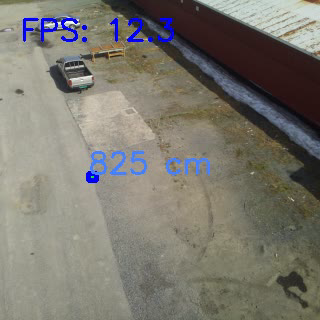
\includegraphics[width=\textwidth]{fig/drone/drone_airshot_1p.png}
    \caption{Photo taken from drone's perspective doing object detection}
\end{figure}